% !TeX root = ../main.tex
\documentclass[./../main.tex]{subfiles}

\begin{document}

Trong phần này, em sẽ mô tả các tính năng nổi bật nhất của hệ thống mới
mà hệ thống UETWork hiện tại chưa cung cấp cho người dùng.

\hypertarget{hux1ed7-trux1ee3-ngux1b0ux1eddi-duxf9ng-thuux1ed9c-nhiux1ec1u-khoa}{%
\subsection{Hỗ trợ người dùng thuộc nhiều
khoa}\label{hux1ed7-trux1ee3-ngux1b0ux1eddi-duxf9ng-thuux1ed9c-nhiux1ec1u-khoa}}

Với hệ thống UETWork cũ, chỉ người dùng thuộc khoa Công Nghệ Thông Tin mới có thể sử dụng hệ thống. Lý do chính của giới hạn này là hệ thống cũ không được thiết kế để mở rộng cho người dùng thuộc nhiều khoa khác nhau.

Nhằm cải thiện vấn đề này, hệ thống UETWork mới được thiết kế từ đầu để có thể sử dụng cho nhiều khoa. Mỗi khoa sẽ có thể quản lý thông tin của mình như kỳ thực tập, sinh viên, giảng viên, đối tác, ... Những thông tin này sẽ được kiểm soát chặt chẽ để tránh việc các khoa đọc được thông tin của nhau.

Để cài đặt tính năng này, cơ sở dữ liệu đã được thiết kế lại để hỗ trợ dữ liệu từ nhiều khoa. Hơn nữa, hệ thống cài đặt thêm cơ chế để kiểm tra quyền truy cập vào dữ liệu của một khoa, đảm bảo vấn đề truy cập trái phép không diễn ra.

\hypertarget{phuxe2n-quyux1ec1n-trong-hux1ec7-thux1ed1ng}{%
\subsection{Phân quyền trong hệ
thống}\label{phuxe2n-quyux1ec1n-trong-hux1ec7-thux1ed1ng}}

Hệ thống UETWork cũ đã cài đặt tính năng phân quyền với các API endpoint. Tuy nhiên, hệ thống chỉ kiểm tra role của người dùng nhưng không kiểm tra quyền sở hữu tài nguyên. Ví dụ, một người dùng đối tác có thể sửa mọi bài đăng trên hệ thống, không chỉ bài của mình. Sự thiếu sót này có thể gây ảnh hưởng đến bảo mật và an ninh của hệ thống.

Với hệ thống mới, việc phân quyền đã được mở rộng bằng việc kiểm tra quyền sở hữu tài nguyên trước khi cho phép truy cập. Quay lại ví dụ ở trên, người dùng đối tác trong hệ thống mới chỉ có thể sửa bài đăng tuyển dụng do mình viết ra, giúp tăng cường sự an toàn của hệ thống.

\hypertarget{gux1eedi-mail-thuxf4ng-buxe1o-vux1ec1-sux1ef1-kiux1ec7n-truxean-hux1ec7-thux1ed1ng}{%
\subsection{Gửi mail thông báo về sự kiện trên hệ
thống}\label{gux1eedi-mail-thuxf4ng-buxe1o-vux1ec1-sux1ef1-kiux1ec7n-truxean-hux1ec7-thux1ed1ng}}

Với một hệ thống mà người dùng cần hoàn thành một công việc nào đó nhanh và hiệu quả nhất có thể, tính năng thông báo là không thể thiếu để đảm bảo người dùng biết cần làm gì tiếp theo.

Hệ thống cũ đã giải quyết vấn đề này bằng cách gửi thông báo trong ứng dụng. Hình \ref{fig:old_notification_page} mô tả màn hình thông báo của hệ thống cũ. Như dễ thấy trên hình, hệ thống có thông báo những sự kiện quan trọng như "xác nhận công ty thực tập", "công ty không được chấp nhận", "thông tin giảng viên", ... Tuy nhiên, với hướng làm gửi thông báo trong ứng dụng, người dùng sẽ phải kiểm tra ứng dụng thường xuyên và dễ bị bỏ qua thông báo.

Để cải thiện nhược điểm này, hệ thống mới cài đặt tính năng thông báo qua email. Một email thông báo tiêu chuẩn sẽ bao gồm những thông tin sau:

\begin{enumerate}
  \item Lý do người dùng nhận được thông báo
  \item Hành động cần thực hiện tiếp theo (nếu có)
  \item Một nút/đường dẫn đưa người dùng tới trang để thực hiện hành động đó
\end{enumerate}

Email này sẽ được gửi để (1) xác nhận một hành động của người dùng và (2) thông báo cho người dùng về một sự kiện đã diễn ra trên hệ thống. Bằng cách này, khả năng người dùng bị bỏ qua thông báo hoặc không biết cần làm gì sẽ giảm xuống đáng kể. Các sự kiện được thông báo bao gồm:

\begin{itemize}
\item
  Chào mừng người dùng tới hệ thống
\item
  Đặt lại mật khẩu
\item
  Sinh viên đăng ký công ty thành công
\item
  Sinh viên đỗ / trượt phỏng vấn
\item
  Sinh viên được chấm điểm
\item
  Công ty được nhà trường xét duyệt thành công
\item
  Sinh viên chọn công ty thành công
\end{itemize}

% TODO: add mail screenshot image
Hình \ref{fig:welcome_mail} và \ref{fig:pass_mail} mô tả 2 email được gửi đi bởi hệ thống. Hình \ref{fig:welcome_mail} là một email đơn giản, bao gồm nội dung và một tài liệu tham khảo. Còn hình \ref{fig:pass_mail} là một email phức tạp hơn, chứa 3 phần nội dung được mô tả ở trên.

\begin{figure}[]
	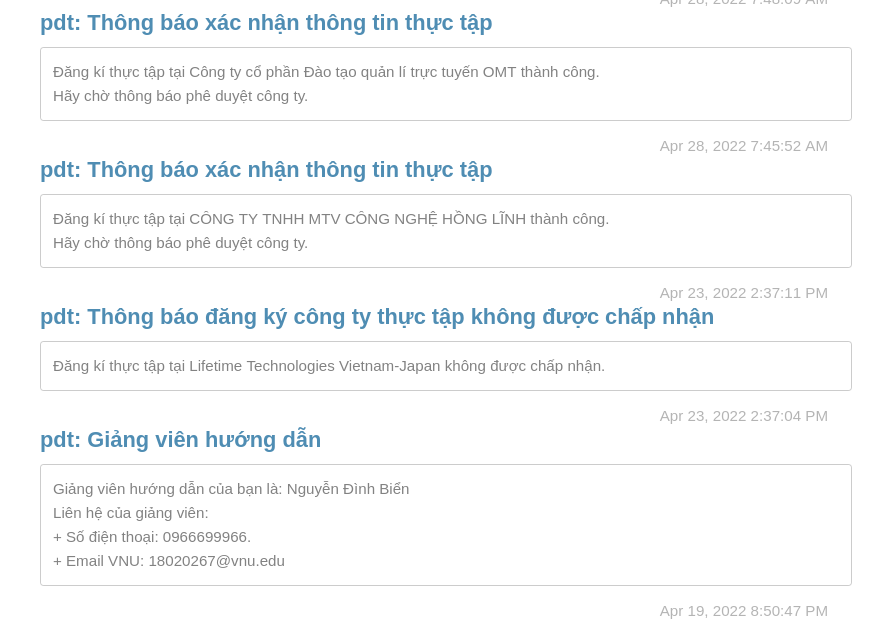
\includegraphics[width=\linewidth]{./images/notification_old.png}
	\caption{Màn hình thông báo của hệ thống cũ}
	\label{fig:old_notification_page}
\end{figure}

\begin{figure}
  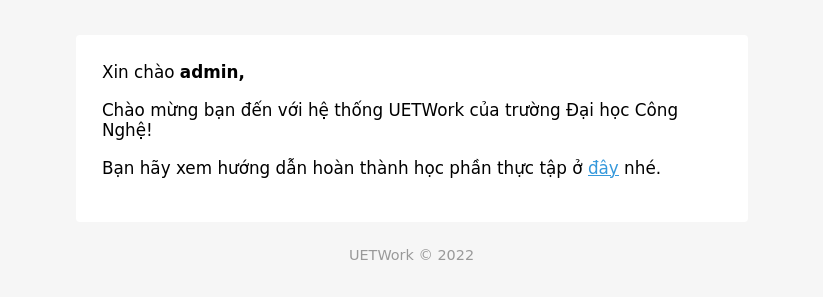
\includegraphics[width=\linewidth]{./images/mail_screenshot.png}
	\caption{Mail chào mừng người dùng}
	\label{fig:welcome_mail}
\end{figure}

\begin{figure}
  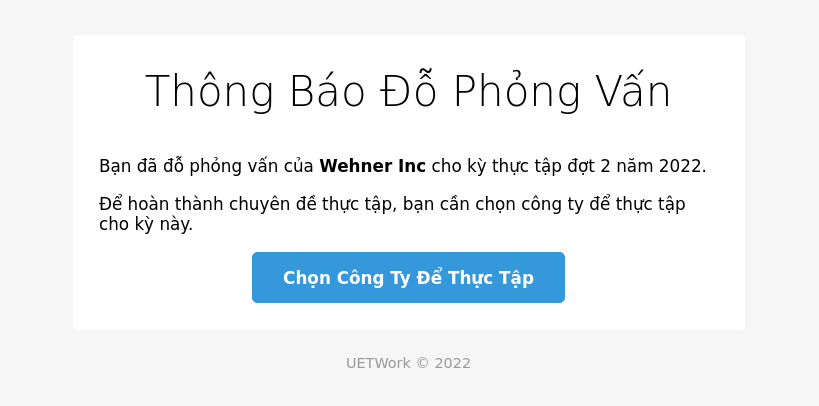
\includegraphics[width=\linewidth]{./images/complex_mail_screenshot.png}
	\caption{Mail thông báo đỗ phỏng vấn}
	\label{fig:pass_mail}
\end{figure}

\hypertarget{thux1ed1ng-kuxea-dux1eef-liux1ec7u}{%
\subsection{Thống kê dữ
liệu}\label{thux1ed1ng-kuxea-dux1eef-liux1ec7u}}

Hệ thống UETWork cũ đã phục vụ nhu cầu quản lý thực tập của nhà trường khá tốt, tuy nhiên, một nhu cầu chưa được thỏa mãn là nhu cầu thống kê dữ liệu.

Để phục vụ nhu cầu thống kê và trực quan hóa dữ liệu, hệ thống UETWork mới cung cấp một dashboard cho người dùng giảng viên, công ty và quản trị viên. Dashboard này sẽ hiển thị con số thống kê có ích cho người dùng, ví dụ như:

\begin{itemize}
\item
  
  Hiển thị số sinh viên tham gia thực tập trong kỳ gần nhất (quản trị
  viên)
  
\item
  
  Hiển thị số bài đăng của kỳ thực tập gần nhất (quản trị viên)
  
\item
  
  Hiển thị số sinh viên đang hướng dẫn (giảng viên)
  
\item
  
  Hiển thị số yêu cầu thực tập (công ty)
  
\end{itemize}

Với dashboard này, người dùng có thể nhìn được các thông số quan trọng nhanh chóng và đưa ra hành động kịp thời.

\hypertarget{ux111a-nguxf4n-ngux1eef-1}{%
\subsection{Đa ngôn ngữ}\label{ux111a-nguxf4n-ngux1eef-1}}

Hệ thống cũ chưa hoàn thiện tốt về mặt ngôn ngữ do giao diện chứa cả tiếng Anh và tiếng Việt, khiến trải nghiệm người dùng không nhất quán. Hình \ref{fig:old_admin_page} cho thấy màn hình quản trị viên của hệ thống cũ. Ở đây, phần sidebar được viết hoàn toàn bằng tiếng Anh, nhưng phần content lại được viết bằng tiếng Việt.

\begin{figure}[]
	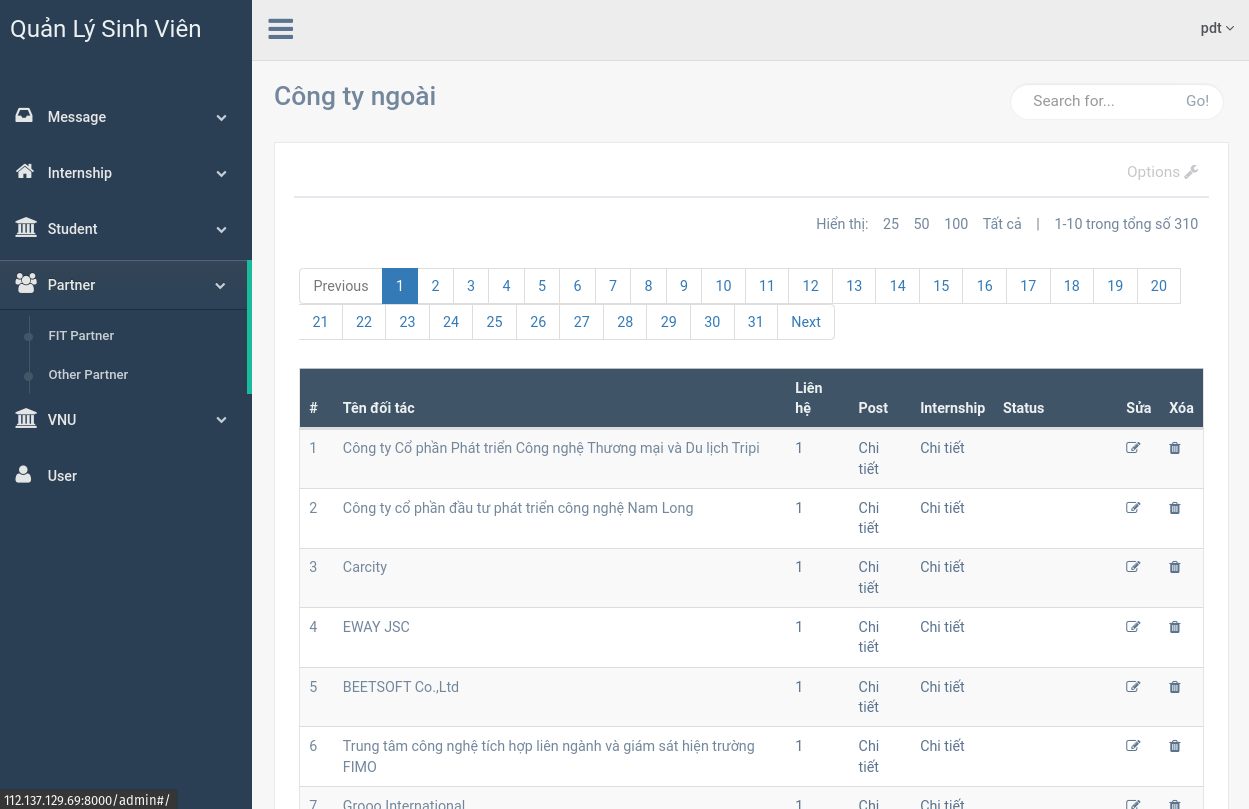
\includegraphics[width=\linewidth]{./images/old_admin_page.png}
	\caption{Màn hình quản trị viên của hệ thống cũ}
	\label{fig:old_admin_page}
\end{figure}

Hệ thống mới đã đặt mục tiêu hỗ trợ đa ngôn ngữ từ thời điểm ban đầu. Trên giao diện, ngườ dùng có thể lựa chọn ngôn ngữ phù hợp nhất với bản thân. Với tính năng này, sinh viên quốc tế có thể sử dụng hệ thống dễ dàng hơn.

Để làm được việc này, phần client sử dụng thư viện i18next\footnote{\url{https://www.i18next.com/}}, cho phép nhà phát triển tạo ra một file chứa toàn bộ nội dung được dịch.

Hình \ref{fig:en_page} và \ref{fig:vi_page} mô tả 2 màn hình tiếng Anh và tiếng Việt của hệ thống.

\begin{figure}[]
	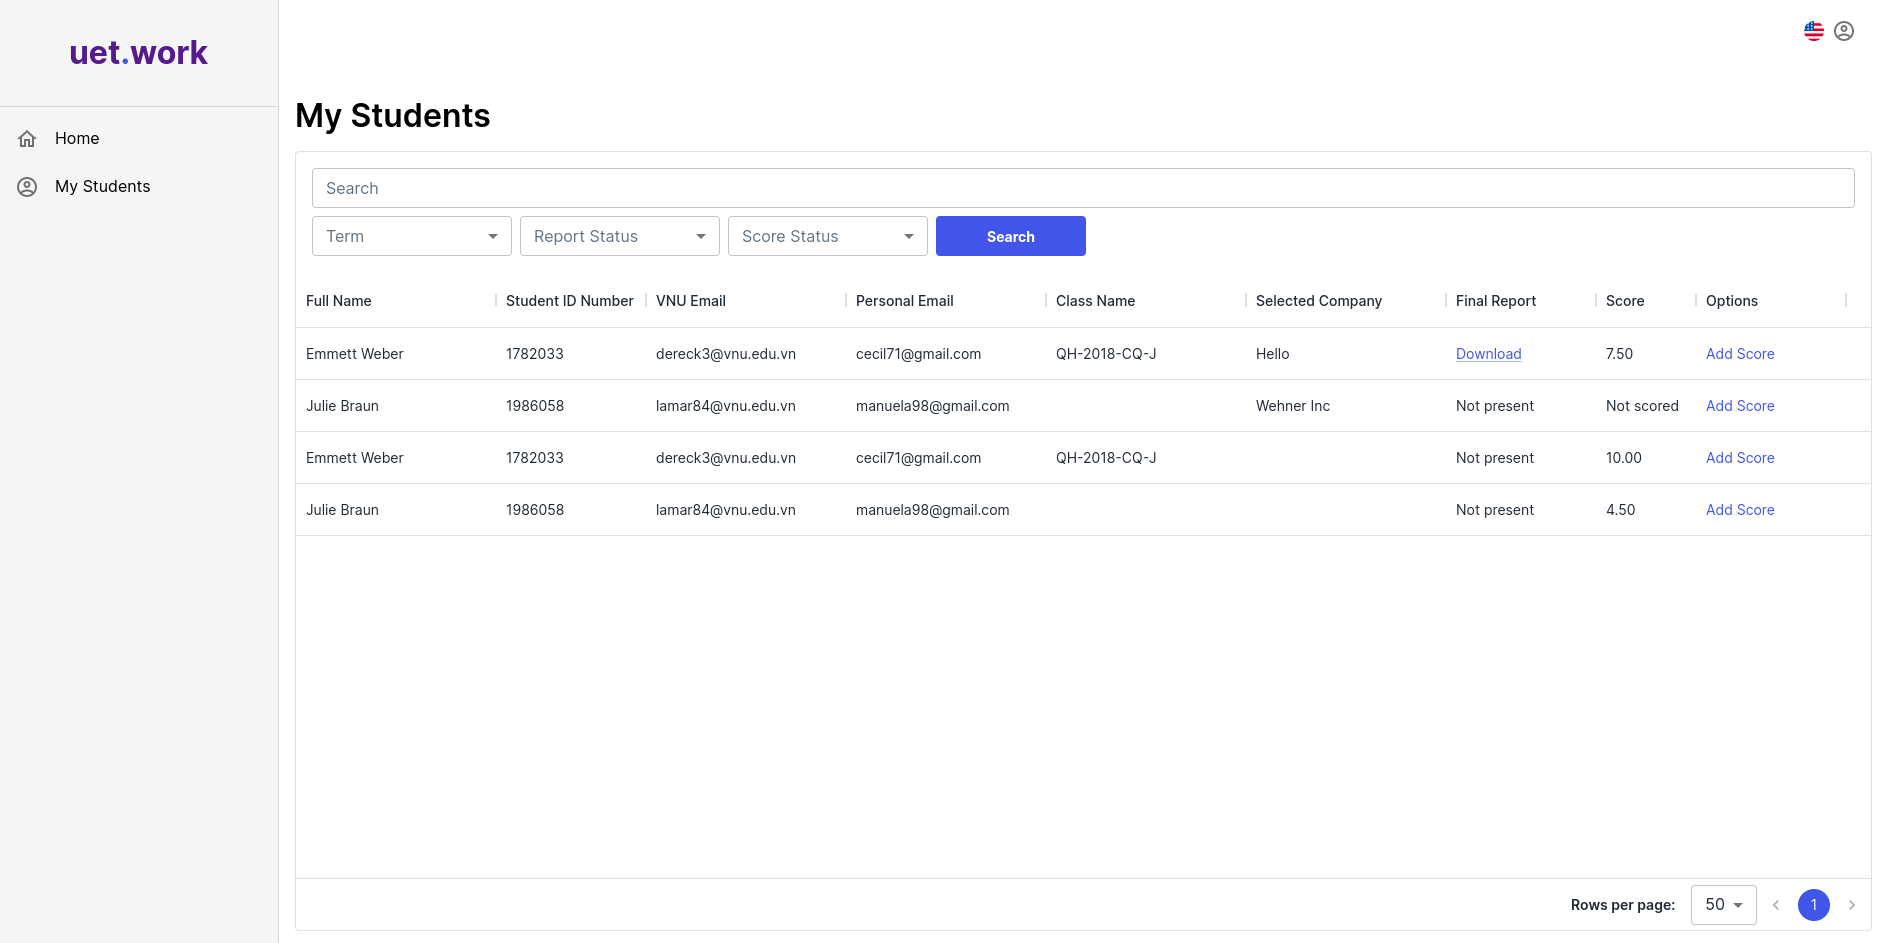
\includegraphics[width=\linewidth]{./images/image13.png}
	\caption{Màn hình hệ thống (tiếng Anh)}
	\label{fig:en_page}
\end{figure}

\begin{figure}[]
	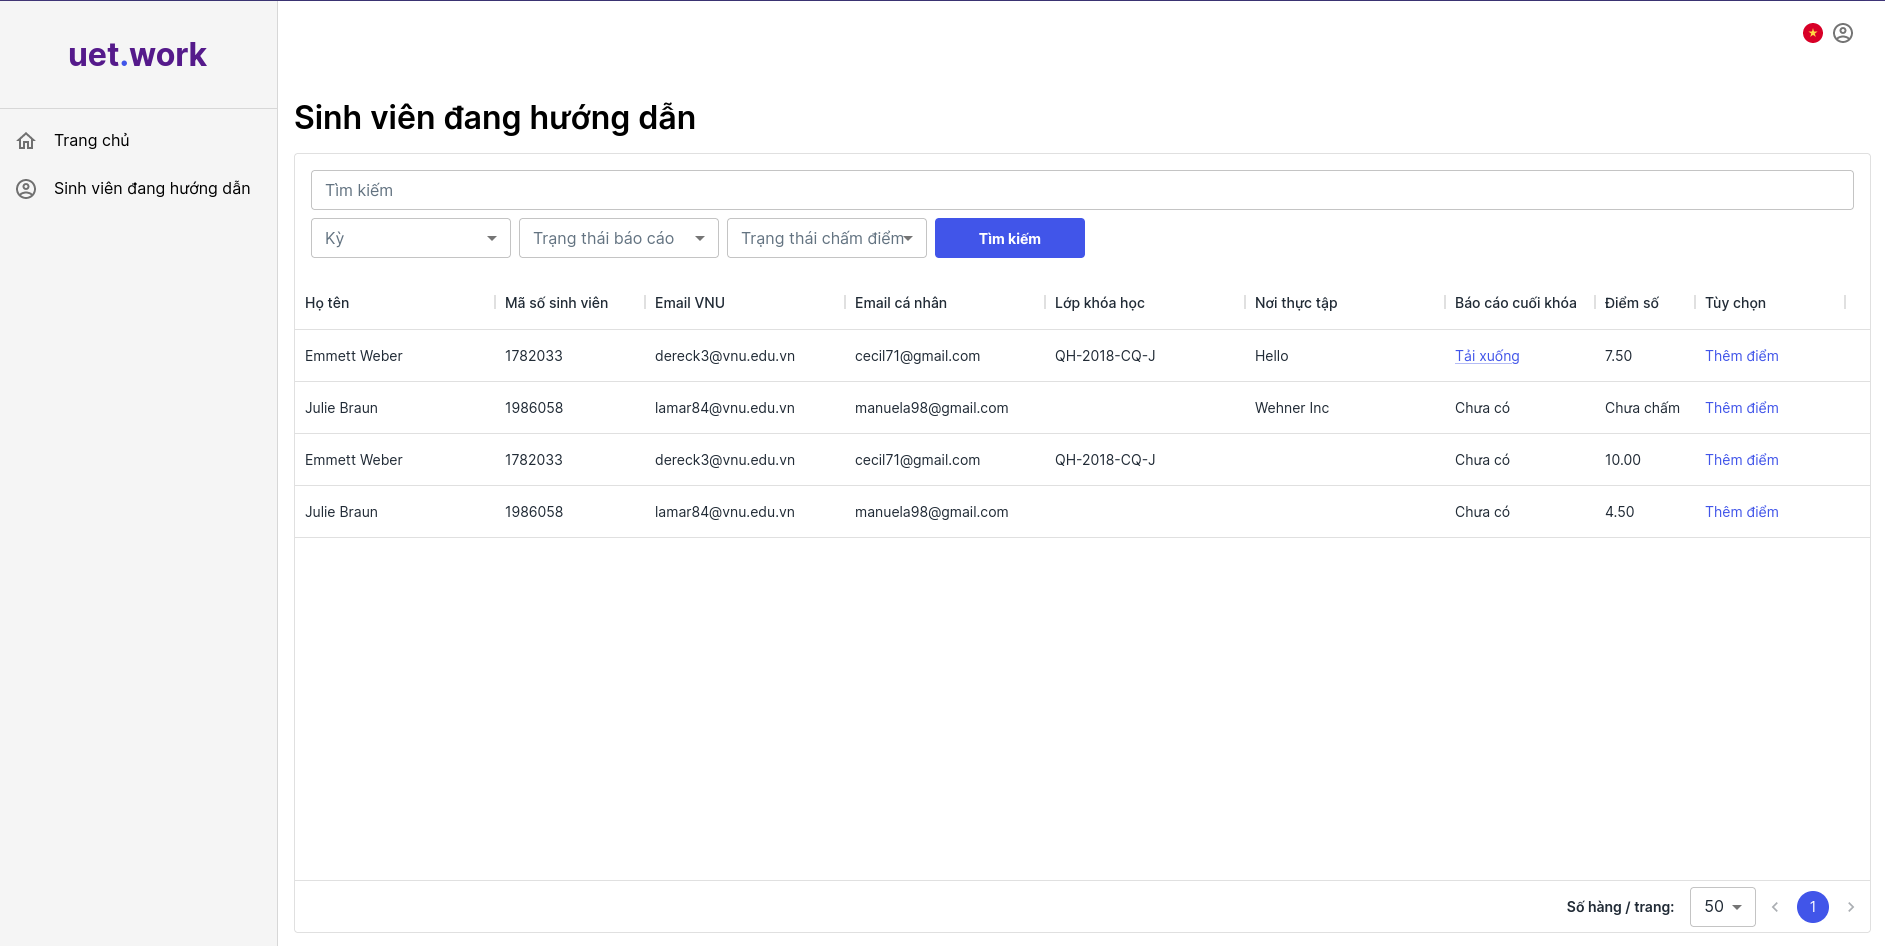
\includegraphics[width=\linewidth]{./images/image12.png}
	\caption{Màn hình hệ thống (tiếng Việt)}
	\label{fig:vi_page}
\end{figure}

\end{document}